
\newcommand{\projectionsWidth}{0.2\textwidth}

\begin{figure}[h]
    	\centering
%    \bgroup
%    \setlength{\tabcolsep}{1mm}
%    \def\arraystretch{2}
%    \adjustbox{max width=0.92\textwidth}{%
%    \begin{tabular}{cccc}
%    \multicolumn{4}{c}{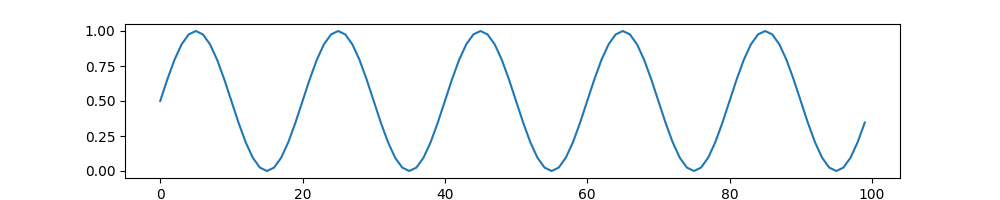
\includegraphics[width=0.95\textwidth, trim={2cm 0cm 2cm 0cm}]{img/projections/signal.png}} \\
%        \fbox{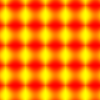
\includegraphics[width=\projectionsWidth]{img/projections/GramianAngularFieldDifference.png}}
%         & \fbox{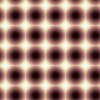
\includegraphics[width=\projectionsWidth]{img/projections/GramianAngularFieldSummation.png}}
%         & \fbox{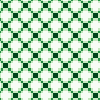
\includegraphics[width=\projectionsWidth]{img/projections/MarkovTransitionField.png}}
%         & \fbox{
\includegraphics[width=\projectionsWidth]{img/projections/RecurrencePlot.png}}\\
%        \fbox{
\includegraphics[width=\projectionsWidth]{img/projections/PoincatePlotLogarithmGrid.png}}
%        & \fbox{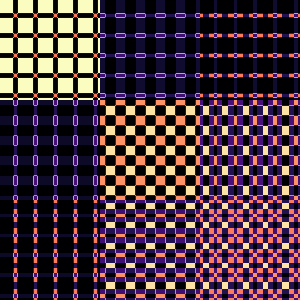
\includegraphics[width=\projectionsWidth]{img/projections/MultiscaleMarkovTransitionField.png}}
%        & \fbox{
\includegraphics[width=\projectionsWidth, height=\projectionsWidth]{img/projections/ShortTimeFFT.png}}
%        & ~ \\
%    \end{tabular}
%    }
%    \egroup
%   	\caption[A signal and its various projection obtained by several methods.]{A signal and its various projection obtained by several methods. In the first line, from the left to the right, the methods are: Gramian Angular Diference Field~\cite{gaf-mtf-1}, Gramian Angular Summation Field~\cite{gaf-mtf-1}, Markov Transition Field~\cite{gaf-mtf-1} and Recurrence Plot~\cite{rp-1}. The methods of the second line are, from the left to the right: Poincaré Plot Density Map~\cite{ecg-6}, Multiscale Markov Transition Field~\cite{imaging-6} and Short Time Fourier Transform Spectogram~\cite{STFT, imaging-1}.}
	\subfigure[]{
		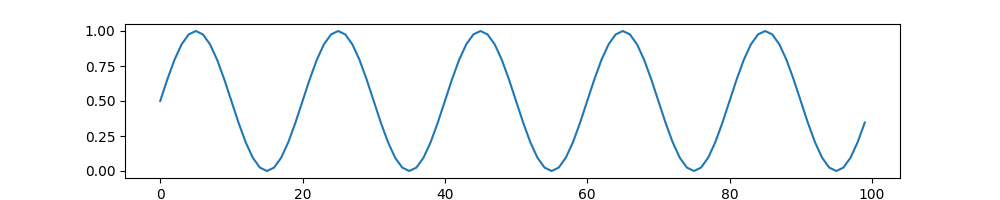
\includegraphics[width=0.95\textwidth]{img/projections/signal.png}
		\label{fig:projections:signal}
	}\\
	\subfigure[]{
		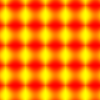
\includegraphics[width=\projectionsWidth]{img/projections/GramianAngularFieldDifference.png}
		\label{fig:projections:GramianAngularFieldDifference}
	}
	\subfigure[]{
		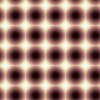
\includegraphics[width=\projectionsWidth]{img/projections/GramianAngularFieldSummation.png}
		\label{fig:projections:GramianAngularFieldSummation}
	}
	\subfigure[]{
		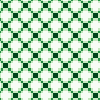
\includegraphics[width=\projectionsWidth]{img/projections/MarkovTransitionField.png}
		\label{fig:projections:MarkovTransitionField}
	}
	\subfigure[]{
		
\includegraphics[width=\projectionsWidth]{img/projections/RecurrencePlot.png}
		\label{fig:projections:RecurrencePlot}
	}\\
	\subfigure[]{
		
\includegraphics[width=\projectionsWidth]{img/projections/PoincatePlotLogarithmGrid.png}
		\label{fig:projections:PoincatePlotLogarithmGrid}
	}
	\subfigure[]{
		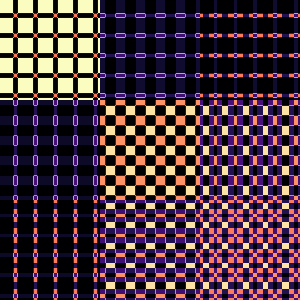
\includegraphics[width=\projectionsWidth]{img/projections/MultiscaleMarkovTransitionField.png}
		\label{fig:projections:MultiscaleMarkovTransitionField}
	}
	\subfigure[]{
		
\includegraphics[width=\projectionsWidth]{img/projections/ShortTimeFFT.png}
		\label{fig:projections:ShortTimeFFT}
	}\\
   	\caption[A signal and its various projection obtained by several methods.]{
   		A signal~\subref{fig:projections:signal} and its various projection obtained by several methods. They are: 
   		\subref{fig:projections:GramianAngularFieldDifference}~Gramian Angular Diference Field~\cite{gaf-mtf-1}, 
   		\subref{fig:projections:GramianAngularFieldSummation}~Gramian Angular Summation Field~\cite{gaf-mtf-1}, 
   		\subref{fig:projections:MarkovTransitionField}~Markov Transition Field~\cite{gaf-mtf-1} and 
   		\subref{fig:projections:RecurrencePlot}~Recurrence Plot~\cite{rp-1}, 
   		\subref{fig:projections:PoincatePlotLogarithmGrid}~Poincaré Plot Density Map~\cite{ecg-6}, 
   		\subref{fig:projections:MultiscaleMarkovTransitionField}~Multiscale Markov Transition Field~\cite{imaging-6} and 
   		\subref{fig:projections:ShortTimeFFT}~Short Time Fourier Transform Spectogram~\cite{STFT, imaging-1}.
   	}
    	\label{fig:literature_projections}
\end{figure}
